\documentclass[a4paper]{article} %%% use \documentstyle for old LaTeX compilers

\usepackage[portuguese]{babel} %%% 'french', 'german', 'spanish', 'danish', etc.
\usepackage{makeidx}
\usepackage{multirow}
\usepackage{multicol}
\usepackage[dvipsnames,svgnames,table]{xcolor}
\usepackage[dvips]{graphicx} 
\usepackage{epstopdf}
\usepackage{ulem}
\usepackage{hyperref}
\usepackage{amsmath}
\usepackage{amssymb}
\usepackage{txfonts}
\usepackage{mathdots}
\usepackage[classicReIm]{kpfonts}

% You can include more LaTeX packages here 

\author{Bruno da silva}

\usepackage[a4paper,top=2.5cm,bottom=2.5cm,left=3cm,right=3cm,marginparwidth=1.75cm]{geometry}

\begin{document}

%\selectlanguage{english} %%% remove comment delimiter ('%') and select language if required


\fontfamily{phv}\selectfont

\begin{center}
	{\Large Universidade Federal Fluminense -UFF}
\end{center}
\begin{center}
	\
\end{center}
\begin{center}
	\
\end{center}
\begin{center}
	\
\end{center}
\begin{center}
	\
\end{center}
\begin{center}
	\
\end{center}
\begin{center}
	\
\end{center}
\begin{center}
	\
\end{center}
\begin{center}
	\
\end{center}
\begin{center}
	\
\end{center}
\begin{center}
	{\Large Oscilador Real
	}
\end{center}
\begin{center}
	\
\end{center}
\begin{center}
	\
\end{center}
\begin{center}
	\
\end{center}

\begin{center}
\end{center}

\begin{center}
	\
\end{center}
\begin{center}
	\
\end{center}
\begin{center}
	\
\end{center}


\begin{center}
	Autor Bruno da Silva Machado
\end{center}
\begin{center}
	\
\end{center}
\begin{center}
	\
\end{center}
\begin{center}
	\
\end{center}
\begin{center}
	\
\end{center}
\begin{center}
	\
\end{center}
\begin{center}
	\
\end{center}

\begin{center}
	\
\end{center}
\begin{center}
	\
\end{center}
\begin{center}
	\
\end{center}
\begin{center}
	Volta Redonda 08 de maio 2017\eject 
	
\end{center}

\setcounter{secnumdepth}{0}
\section{Introdu\c{c}\~{a}o}
\noindent

Neste trabalho, estudamos o oscilador harm\^onico amortecido admitindo uma for\c{c}a de atrito de contato, que depende somente do sinal da velocidade. Usaremos o m\'etodo de Verlet um m\'etodo num\'erico usado para estudar equa\c{c}\~oes do movimento de Newton. \'E frequentemente usado no calculo da trajet\'orias de part\'iculas din\^amicas em simula\c{c}\~oes computacionais.
\noindent \eject 

\section{O oscila\c{c}\~oes reais}
\noindent 
\'E um oscilador massa mola \'e composto por uma mola com massa desprez\'ıvel que obede\c{c}a a lei de Hooke e um corpo de massa m que n\~ao se deforme sob a\c{c}\~ao de qualquer for\c{c}a, posto sobre uma superf\'ıcie com atrito de contato que depende apenas do sinal da velocidade e n\~ao do seu m\'odulo.

\begin{center}
	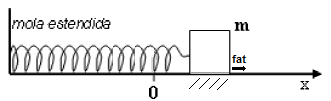
\includegraphics[width=3.31in,height=1.01in,keepaspectratio = false]{mola.png}
	
	\scriptsize Figura 1. sistema massa mola fora da poci\c{c}\~ao de equil\'ibrio. Observe a for\c{c}a de atrito e sempre oposta ao movimento
	
\end{center}

O oscilador, apresentado na figura 1, est\'a sujeito a duas for\c{c}as:

a) uma for\c{c}a restauradora dada pela lei de Hooke (f = -kx) onde k \'e a constante el\'astica da mola e x \'e o deslocamento medido em rel\c{c}\~ao \'a posi\c{c}\~ao em quea mola n~ao est\'a esticada ou comprimida;

b) uma for\c{c}a dissipativa que \'e sempre contr\'aria ao movimento do bloco. Esta for\c{c}a tem uma descontinuidade quando a velocidade $(\dot{x})$ se anula. Para $\dot{x} \neq 0$ o m\'odulo da for\c{c}a de atrito pode ser escrito como:
\[fa = \mu_cN = \mu_cmg (1)\]
onde $\mu_c$ \'e o coeficiente de atrito cin\'etico e N \'e a for\c{c}a normal \'a superf\'icie.

Como a for\c{c}a de atrito \'e contr\'aria ao movimento, teremos duas equa\c{c}\~oes distintas para $\dot{x} \neq 0$, dadas pela 2$^circ$ lei de Newton $F = m\ddot{x}$:

\[m\ddot{x} + kx = + \mu_cmg\] se $\dot{x} < 0$
\[m\ddot{x} + kx = - \mu_cmg\] se $\dot{x} > 0$(2)

\section{Solu\c{c}\~ao do oscilador}

As equa\c{c}\~oes ateriores s\~ao equa\c{c}\~oes diferenciais lineares n\~ao homog\^eneas que pode ser solucionadas.
partindo da equa\c{c}\~o homog\^enea nos temos:

\[m\ddot{x} + kx = 0\]
\[m\ddot{x} = - kx\]
\[\ddot{x} = -\frac{kx}{m}\]
Veja que \'e uma EDO de 2$^circ$ ordem com coeficientes constantes. Aplicando a equa\c{c}\~ao caracter\'isticas da EDO temos:
\[r^2 = -\frac{kx}{m}\] 
\[r = \pm \sqrt{-\frac{kx}{m}}\]
\[r = \pm \sqrt{\frac{kx}{m}}i\]
logo a solu\c{c}\~ao \'e $x(t) = e^r \rightarrow e^{\pm \sqrt{\frac{kx}{m}}i}$, cujo aplicando a formula de Euler obtemos:
\[x(t) = A\cos(\omega{t} + \phi)\]

A solu\c{c}\~ao particular pode ser obtida por integra\c{c}\~ao ou por substitui\c{c}\~ao de uma solu\c{c}\~ao tentativa na equa\c{c}\~ao diferencial. Em geral, a solu\c{c}\~ao particular tem um comportamento semelhante ao termo n~ao homog\^eneo, neste caso uma constante. Supondo $x_p = \pm D$ onde D \'e uma constante, substituindo na equa\c{c}\~ao (2) obtemos:
\[D = \frac{\mu_cg}{\omega^2}\] (3)
Portanto, a solu\c{c}\~ao geral \'e dada por:
\[x(t) = A\cos(\omega{t} + \phi) \pm \frac{\mu_cg}{\omega^2}\]
onde o \'indice (+) corresponde a $\dot{x} < 0$ e o \'indice (-) a $\dot{x} > 0$. Derivando em relac\c{c}\~ao ao tempo obtemos:
\[v(t) = \dot{x} = -A\omega\sin(\omega{t} + \phi) \](4)

\paragraph{\textit{O m\'etodo de Verlet}} A primeira vista \'e comum calcular trajet\'orias usado o m\'etodo de Euler. Contudo, este tipo de integral que sofre alguns problemas, o  m\'etodo de Euler n\~ao funciona para um problema to simples quanto o oscilador harm\^onico, independentemente de quo pequeno seja o espa\c{c}o de tempo. Estabilidade da t\'ecnica depende bastante da taxa de atualiz\c{c}\~ao, ou a capacidade de identificar com preciso as posi\c{c}\~oes em uma pequena vari\c{c}\~ao de tempo. O m\'etodo de Verlet uma importante ferramenta, capaz de resolver um grande n\'umero de problemas que no possuem uma solu\c{c}\~ao analtica.

\[v_{t+1} = v_t + a_t\Delta{t}/2\]
\[x_{t+1} = x_t + v_{t+1/2} + a_{t+1}\Delta{t}/2 \pm \frac{\mu_cg}{\omega^2}\]
\[V_{t+1} = V_{t+1/2} + a_{t+1}\Delta{t}/2 \]
que pode ser reescrito como:
\[x_{t+1} = x_t + v_tt+a_t(\delta{t})^2/2 \pm \frac{\mu_cg}{\omega^2}\]
\[v_{t+1} = v_t + 1/2(a_{t+1}+a_t)\Delta{t}\](5)

\section{Resultado}

Nas figuras a seguir vamos visualizar as solu\c{c}\~oes obtidas na se\c{c}\~ao anterior, nelas est\~ao representadas a posi\c{c}\~ao, velocidade e acelera\c{c}\~ao do oscilador para o caso em que frequ\^encia angular $w = 2,23$rad/s, com o coeficiente de atrito cin\'etico $\mu_c = 0,003$ e a amplitude $x_0 = 3$m. Nestes
gr\'aficos, podemos notar que a posi\c{c}~ao e a velocidade s\~ao cont\'inuas embora a modula\c{c}~ao da amplitude n\~ao seja,Tamb\'em notamos que suas amplitudes decrescem linearmente com o tempo, o que torna ele um oscilador linearmente amortecido.

\begin{center}
	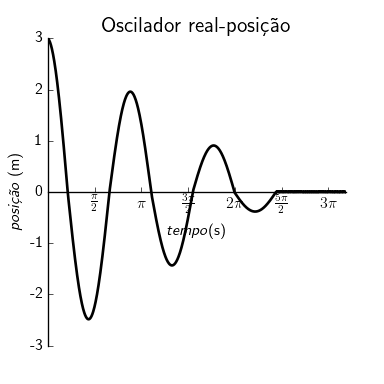
\includegraphics[width=3.84in,height=3.84in,keepaspectratio = false]{image1_1.png}
	
	\scriptsize Figura 2. Gr\'afico da Posi\c{c}\~ao x Tempo do oscilador - A linha cont\'inua representa a oscila\c{c}\~ao do corpo, que se mant\'em at\'e que a for\c{c}a feita pela mola em um ponto de retorno seja menor que a for\c{c}a de atrito est\'atico m\'axima.
	
\end{center}

\begin{center}
	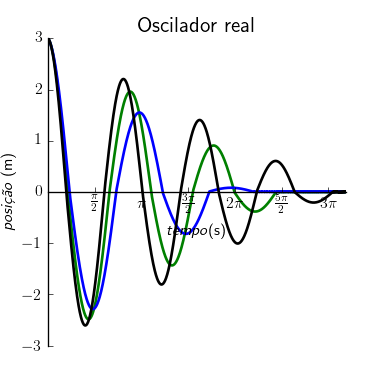
\includegraphics[width=3.84in,height=3.84in,keepaspectratio = false]{image_c1.png}
	
	\scriptsize Figura 3. Gr\'afico da Posi\c{c}\~ao x Tempo do oscilador partindo com a mesma amplitude porem com velocidade angular distintas- A linha cont\'inua representa a oscila\c{c}\~ao do corpo, que se mant\'em at\'e que a for\c{c}a feita pela mola em um ponto de retorno seja menor que a for\c{c}a de atrito est\'atico m\'axima. Observe as mudan\c{c}as no comportamento do per\'iodo e da amplitude em compara\c{c}\~ao com o OHS
	
\end{center}

\begin{center}
	
	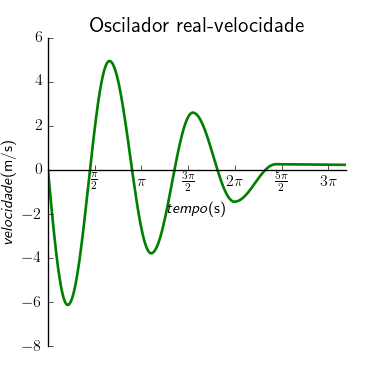
\includegraphics[width=3.84in,height=3.84in,keepaspectratio = false]{image1_2.png}
	
	\scriptsize Gr\'afico da Velocidade x Tempo do oscilador - Podemos notar que a velocidade m\'axima em cada semi-ciclo decresce linearmente com o tempo, tem a forma senoidal e a mudan\c{c}a de amplitude ocorre nos pontos em que a velocidade \'e nula.
\end{center}
 
\begin{center}
	
	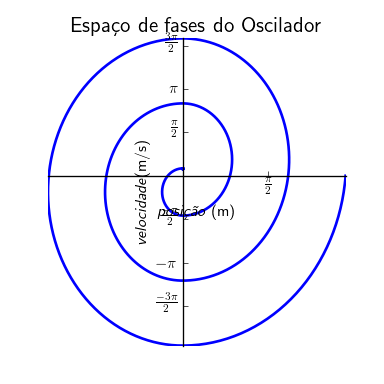
\includegraphics[width=3.84in,height=3.84in,keepaspectratio = false]{image1_3.png}
	
	\scriptsize espa\c{c}o de fase do oscilador linearmente amortecido a patir dele podemos supor que a energia do oscilador n\~ao se conserva uma vez que a curva n\~ao fechada e tem um formato de espiral.
\end{center}

Agora vamos verificar a se depend\^encia da amplitude e do per\'iodo com a for\c{c}\~a de atrito. Para isso vamos supor um oscilador na lua partindo com as mesmas codi\c{c}\~oes iniciais do exemplo anterior.

\begin{center}
	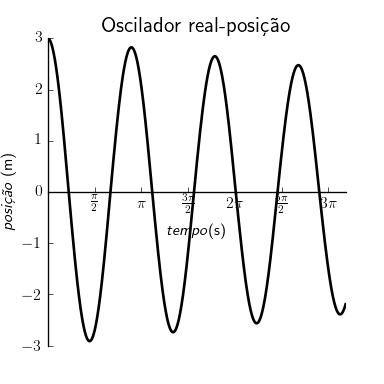
\includegraphics[width=3.84in,height=3.84in,keepaspectratio = false]{image2_1.png}
	
	\scriptsize Figura 2. Gr\'afico da Posi\c{c}\~ao x Tempo do oscilador na lua - a oscila\c{c}\~ao do corpo se mant\'em at\'e que a for\c{c}a feita pela mola em um ponto de retorno seja menor que a for\c{c}a de atrito est\'atico m\'axima. Observe o aumento da amplitude em compara\c{c}\~ao a terra.
	
\end{center}

\begin{center}
	
	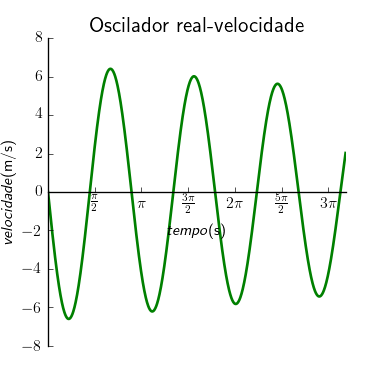
\includegraphics[width=3.84in,height=3.84in,keepaspectratio = false]{image2_2.png}
	
	\scriptsize Gr\'afico da Velocidade x Tempo do oscilador na lua - Podemos notar que a velocidade m\'axima em cada semi-ciclo decresce linearmente com o tempo, tem a forma senoidal e a mudan\c{c}a de amplitude ocorre nos pontos em que a velocidade \'e nula o que se mostra uma caracter\'istica deste tipo de movimento. Note tamb\'em que a velocidade diminui mais lentamente em compara\c{c}\~ao com oscilador naa terra.  
\end{center}

\begin{center}
	
	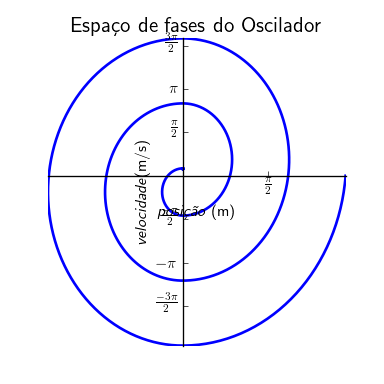
\includegraphics[width=3.84in,height=3.84in,keepaspectratio = false]{image1_3.png}
	
	\scriptsize espa\c{c}o de fase do oscilador linearmente amortecido na lua a patir dele podemos tamb\'em supor que a energia do oscilador n\~ao se conserva uma vez que a curva n\~ao fechada e tem um formato de espiral que decresce bem devagar.
\end{center}
 
\begin{center}
 	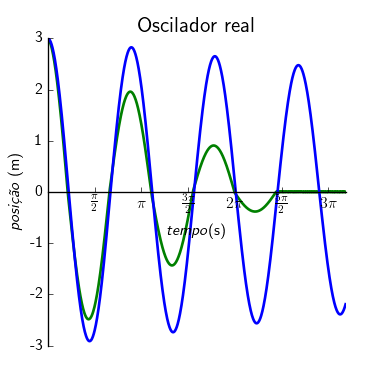
\includegraphics[width=3.84in,height=3.84in,keepaspectratio = false]{image_c0.png}
 	
 	\scriptsize Figura 3. Gr\'afico comparando a Posi\c{c}\~ao x Tempo do oscilador na terra com o na lua partindo com as mesma condi\c{c}\~oes iniciais observe que a uma diferen\c{c}a significativa entre as amplitude porem o per\'iodo se manteve o mesmo.
 	
\end{center}

A partir desses exemplos vemos que a amplitude depende da for\c{c}a de atrito mas o per\'iodo não.

Utilizando a equa\c{c}\~ao de onda podemos ver isso.
\[\frac{X^2}{A^2} + \frac{V^2}{A^2\omega^2} = 1\]

fazendo X = $\cos(\omega{t}+\phi)$ e V = $v(t)$ podemos reescrever X como $X = x(t) - \frac{\mu_cg}{\omega^2}$, substituindo temos:
\[\frac{\left(x- \frac{\mu_cg}{\omega^2}\right)^2}{A^2} + \frac{v^2}{A^2\omega^2} = 1\]
Assim reobtemos a equa\c{c}\~ao de onda mas desta vez deslocada por um fator constante $\frac{\mu_cg}{\omega^2}$, veja que este fator esta associado com a fun\c{c}\~ao x(t) [4] que influencia diretamente a amplitude do oscilador, i.e temos que A = x(0).

E por fim vamos verificar se o per\'iodo depende do atrito e estima -lo no exemplos anteriores. Para isso come\c{c}amos pela posi\c{c}\~ao:

\[x(t) = A\cos(\omega{t} + \phi) \pm \frac{\mu_cg}{\omega^2}\]
sabemos pelo grafico que quando x(t) = 0 v atinge o valor max\'imo e \'e nesses pontos em que podemos calcular o per\'iodo, assim derivando x(t) e igualando a zero

\[-A\omega\sin(\omega{t} + \phi)  = 0\]
neste caso o angulo $\phi$ \'e igual a zero
\[A\omega\sin(\omega{t})  = 0\]
dividindo ambos os lados por $A\omega$
\[\sin(\omega{t}) = 0\]
\[\omega{t} = \arcsin(0)\]
\[\omega{t} = \pi\]
\[t = \frac{\pi}{\omega}\](6)
vimos que quando derivamos x(t) a for\c{c}a de atrito some da equa\c{c}\~oes seguintes de modo que podemos observar que o per\'iodo s\'o depende da velocidade angular, assim conclu\'imos que o per\'iodo n\~ao depende do atrito.
usando a formula (6) podemos estimar t facilmente nos exemplos anteriores
\[t = \frac{\pi}{2,23}s \approx 1,40s\]    
 
 
\section{Conclu\c{c}\~ao}

Nesse trabalho estudamos o comportamento do oscilador real e apresentamos a solu\c{c}\~ao de um oscilador amortecidoem que a for\c{c}a dissipativa depende apenas do sinal de velocidade e n~ao de seu m\'odulo, tambem verificamos que a amplitude depende do atrito mas o per\'iodo não . Fizemos uma analise e vimos os m\'etodos de Verlet que apresenta uma estabilidade em equa\c{c}\~oes diferenciais de 2$^circ$ ordem e bem mais confi\'avel que o Euler-Cromer.

\section{Referencia}

\noindent 
\indent 1. a) D. HALLIDAY e R. RESNICK, Fundamentos de F\'isica, vol. 2, Livros T\'ecnicos e Cient\'ificos, Rio de Janeiro, 1991. b) P. TIPLER, F\'isica, vol. 2, 3a ed., Guanabara Koogan, Rio de Janeiro, 1991.

\indent 2. J. B. MARION, Classical Dynamics, 2a ed., Academic Press, New York, 1965.

\indent 3. M\'etodo de Verlet, Wikip\'edia a enciclop\'edia livre, 2017

\indent 4. Oscilador massa-mola - Movimento Harm\^{o}nico simples, Laifi ,2017


\end{document}

